\chapter{Experimental Results}
\label{ch:expResults}
\begin{chapterquote}{Felix Klein}
"The greatest mathematicians, as Archimedes, Newton, and Gauss, always united theory and applications in equal measure."
\end{chapterquote}

\section{Accuracy and MSE}
In this chapter the results for each model and each experiment are shown. We compared the models using the two criteria explained in the previous chapter. The RNN was trained for just 10 epochs to avoid overfitting as it quickly reached a very low in sample error smaller than 0.01. On the other hand, the ANN was trained for 300 epochs in order to reach approximately the same in sample error as the RNN. 


The MSE and the accuracy scores are shown in Table \ref{table:accmse}. The best performance is where the MSE is the lowest and the accuracy is the highest. It can be noticed in Figure \ref{fig:accmse} that the RNN had the best performance in both cases. The support vector machine got a higher accuracy than the ANN but the last one had a lower MSE.

In this case, the accuracy is measuring the second comparison criteria, meaning, how good is the model to catch the ups and downs of the stock market price. The best models are the RNN and the SVM. On the other hand, the RNN and the ANN are better in predicting the price. Nevertheless, there is a difference of more than 1 point between the MSE of the two models.  

%tabla de accmse
\begin{table}{}
\begin{center}
\begin{tabular}{ c | c | c }
    \hline
     \textbf{Model} &  \textbf{MSE} &    \textbf{Accuracy}\\ \hline
    RNN&  1.66&  0.45 \\ \hline
    SVM&  3.39&  0.44\\ \hline
    ANN&  2.91&  0.41\\ \hline
      \hline
  \end{tabular}
  \caption{MSE and Accuracy of the Models}
 \label{table:accmse}
\end{center}
 \end{table}

%gráfica de accmse
\begin{figure}
\label{fig:accmse}
\center
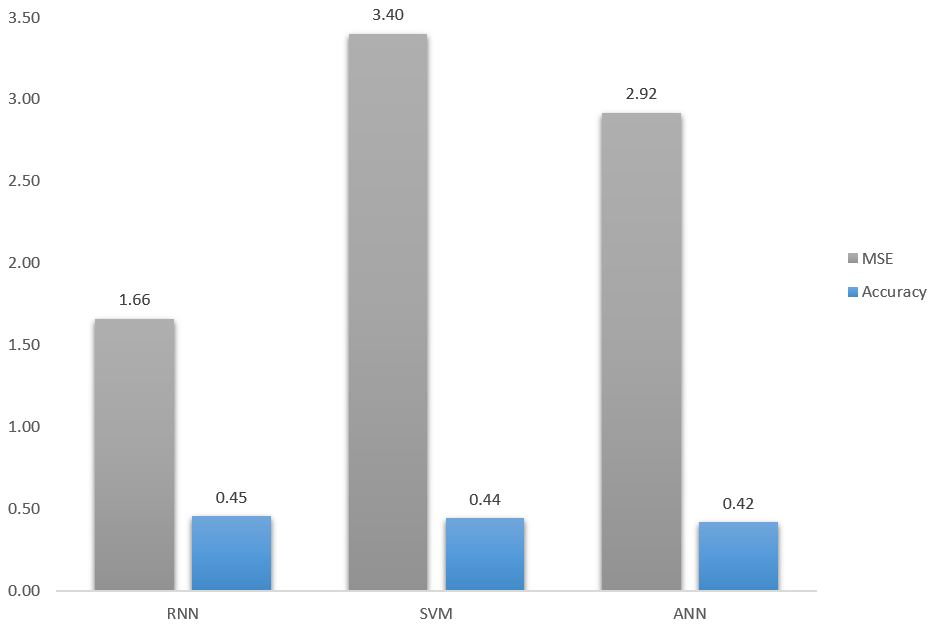
\includegraphics[width=13.5cm,height=8.5cm]{Figures/accmseBar.JPG}
\caption{MSE and Accuracy of each Model}
\end{figure}


\section{Confusion Matrix, Precision, F1 Score}

The confusion matrix, precision, and F1 score correspond to the second comparison criteria and are studied by class: Up, if the actual price is higher than the past one and Down, if it is lower. This analysis is interesting since we can study where each model is better than the other. 

The values in the left to right diagonal of the confusion matrix, are the ones that the model predicted correctly. Conversely, the values out of this diagonal are the ones where the model got the prediction wrong.

As shown in \ref{fig:resultsRNN}, the most of the RNN mistakes are at the upper right, meaning, the true negative values that correspond to the ups of the price. It can be said that the model moved to the right direction in almost half of the times. Although it may seem as a bad performance, the mean of the differences between the actual price and the previous one in the test subset is only 0.5 points. 

On the other hand, the majority of the mistakes of the SVM and the ANN models were at the false positive corner. This case is when the price went down with respect to the previous one and the model moved up. The ANN performed better in this case, but the SVM outperformed the ANN when the price went up.

%resultados RNN
\begin{figure}
\center
\subfloat[RNN Confusion Matrix]{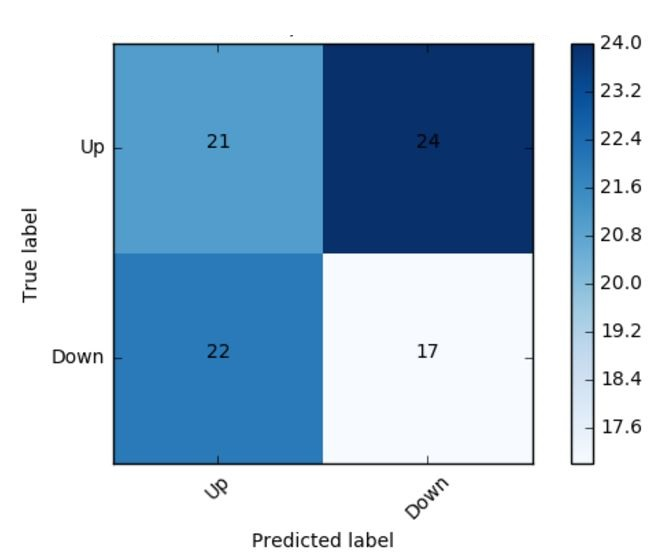
\includegraphics[width=6.5cm,height=5.5cm]{Figures/cmRNN.JPG}} 
\subfloat[RNN Normalized Confusion Matrix]{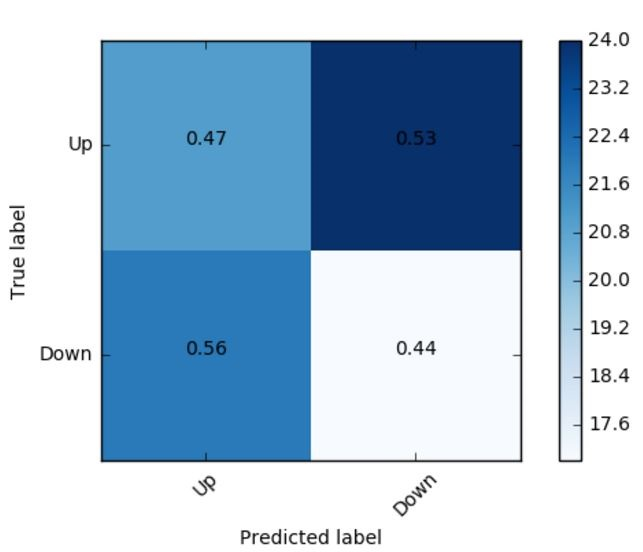
\includegraphics[width=6.5cm,height=5.5cm]{Figures/cmnRNN.JPG}}\\
\subfloat[RNN Classification Report]{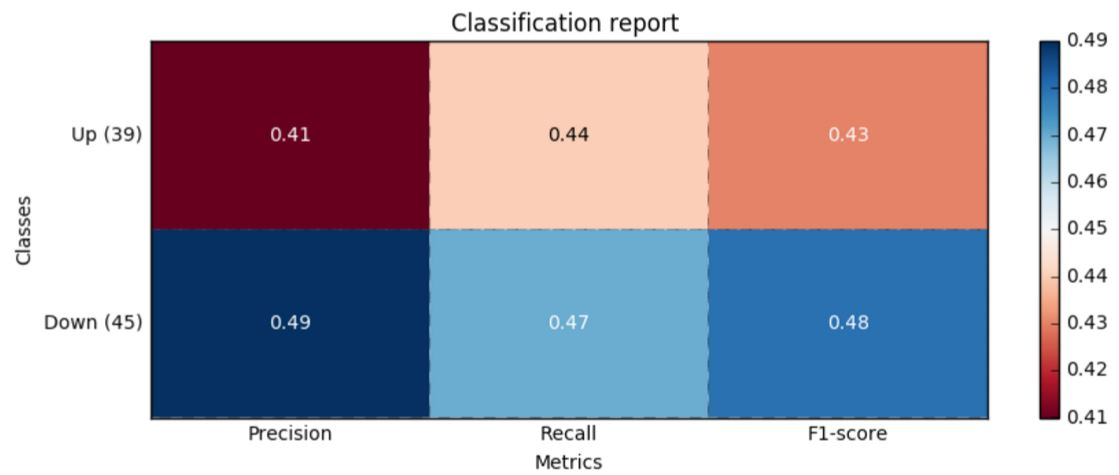
\includegraphics[width=10.5cm,height=5.5cm]{Figures/reportRNN.JPG}}
\caption{RNN Results}
\label{fig:resultsRNN}
\end{figure}

%resultados SVM
\begin{figure}
\center
\subfloat[SVM Confusion Matrix]{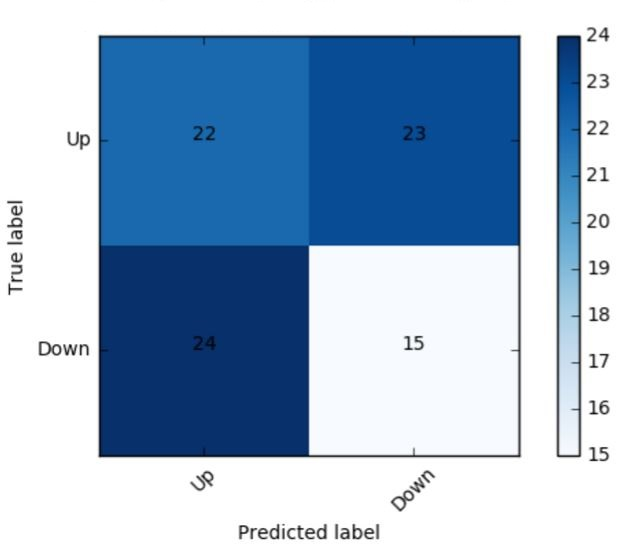
\includegraphics[width=6.5cm,height=5.5cm]{Figures/cmSVM.JPG}} 
\subfloat[SVM Normalized Confusion Matrix]{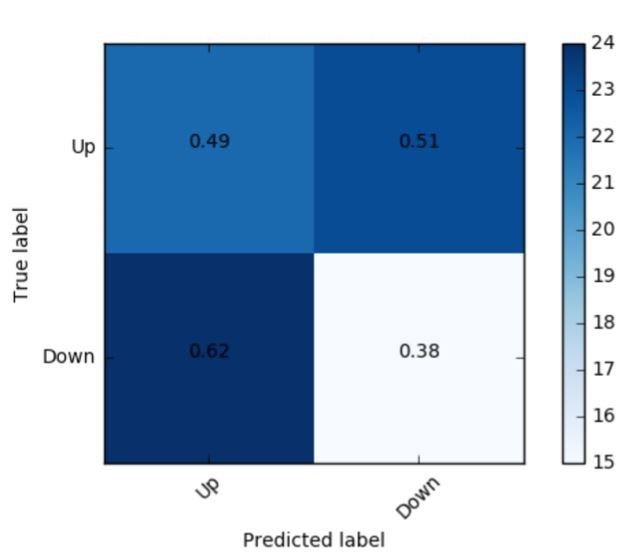
\includegraphics[width=6.5cm,height=5.5cm]{Figures/cmnSVM.JPG}}\\
\subfloat[SVM Classification Report]{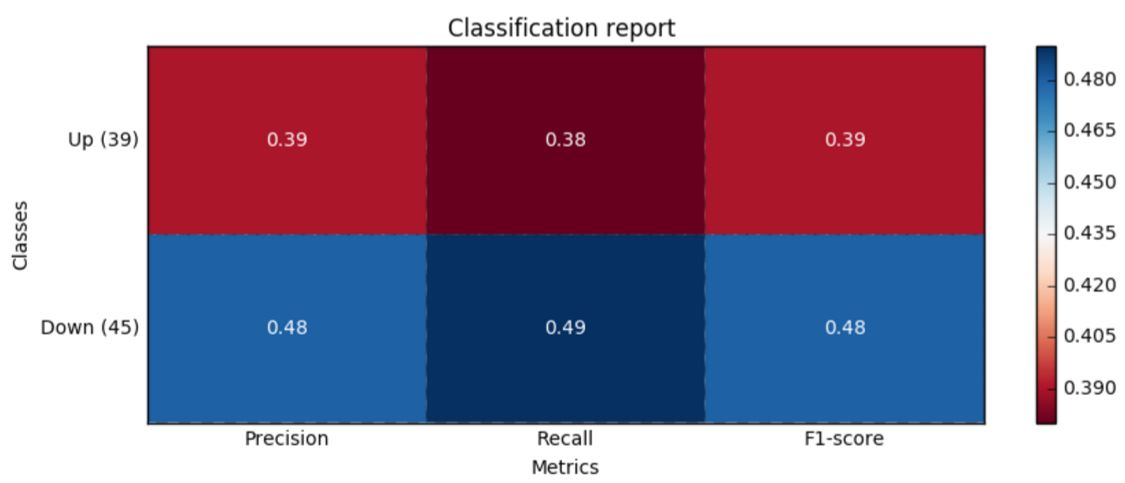
\includegraphics[width=10.5cm,height=5.5cm]{Figures/reportSVM.JPG}}
\caption{SVM Results}
\label{fig:resultsSVM}
\end{figure}

%resultados NN
\begin{figure}
\center
\subfloat[NN Confusion Matrix]{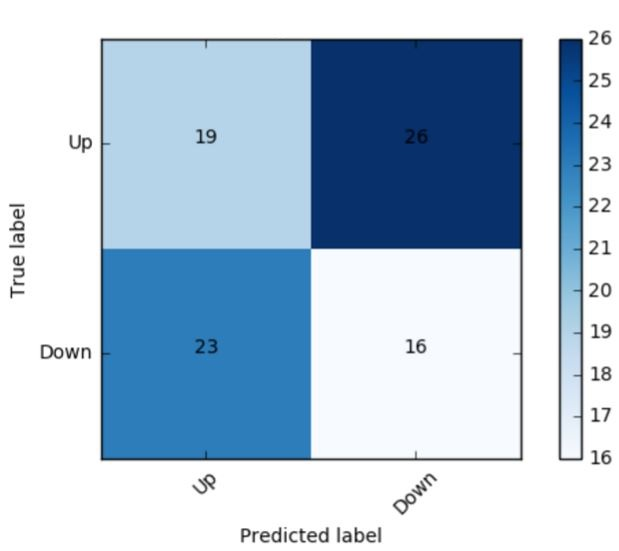
\includegraphics[width=6.5cm,height=5.5cm]{Figures/cmNN.JPG}} 
\subfloat[NN Normalized Confusion Matrix]{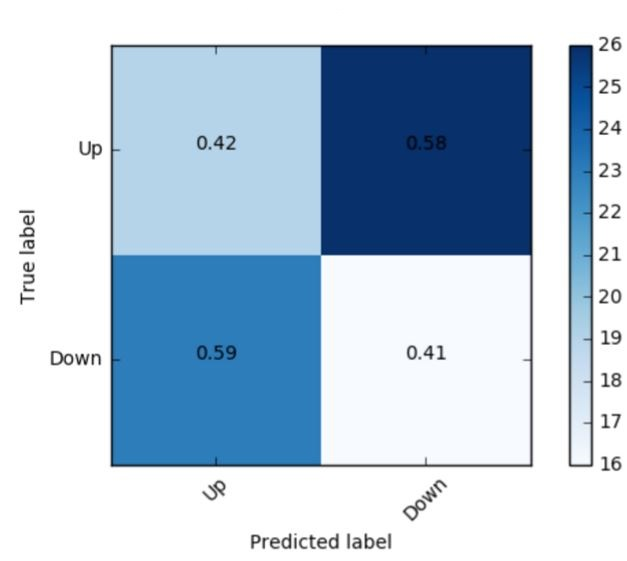
\includegraphics[width=6.5cm,height=5.5cm]{Figures/cmnNN.JPG}}\\
\subfloat[NN Classification Report]{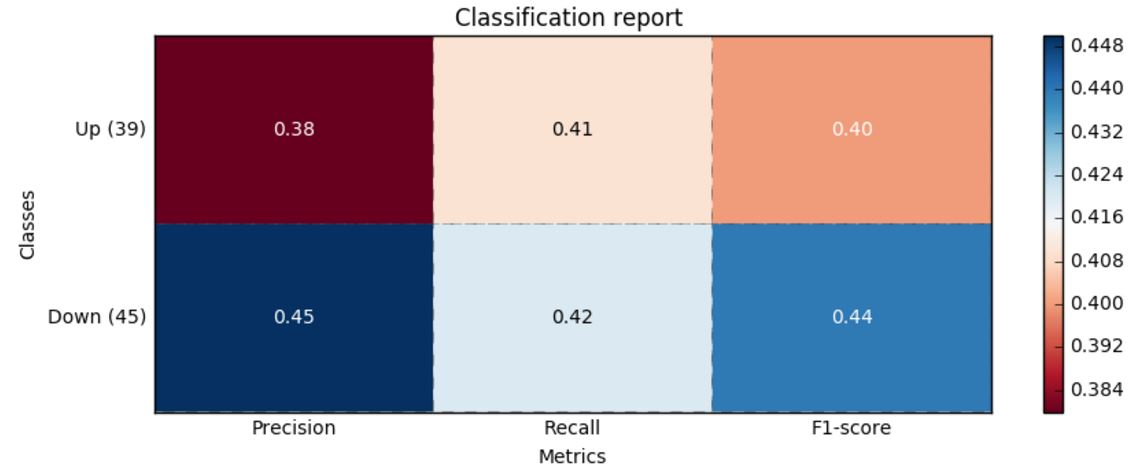
\includegraphics[width=10.5cm,height=5.5cm]{Figures/reportNN.JPG}}
\caption{NN Results}
\label{fig:resultsNN}
\end{figure}

%comparison
\begin{figure}
\center
\subfloat[Precision]{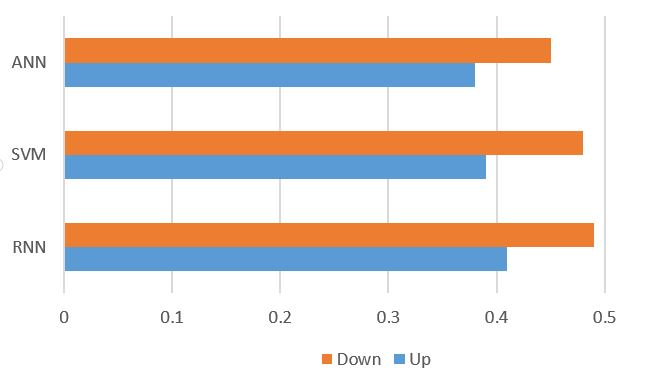
\includegraphics[width=8cm,height=5.5cm]{Figures/precision.JPG}} 
\subfloat[Recall]{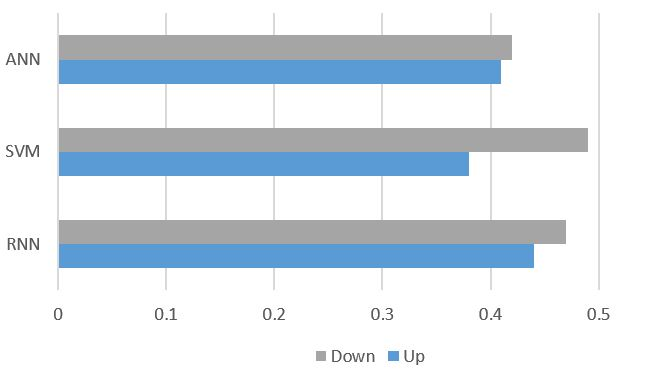
\includegraphics[width=8cm,height=5.5cm]{Figures/recall.JPG}} \\
\subfloat[F1 Score]{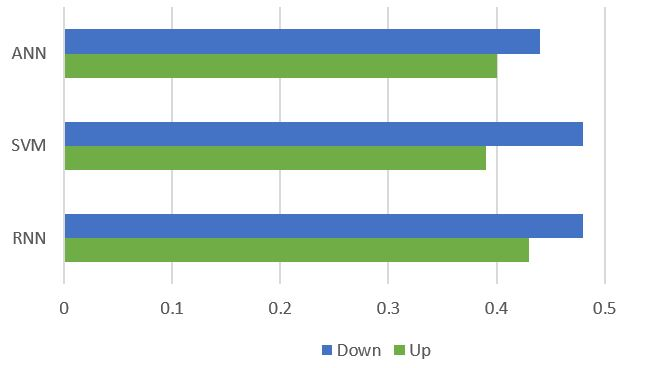
\includegraphics[width=8cm,height=5.5cm]{Figures/F1_Score.JPG}}
\caption{Comparison between ANN, SVM, and RNN}
\label{fig:comparison}
\end{figure}

%Precision
The correct predictions were very balanced in both cases between ups and downs taking into account that the test subset had 6 more downs than ups. The recall graph from figure \ref{fig:comparison}, shows the SVM outperformed the two other models when predicting the downs of the price. Nevertheless, the RNN model was better to predict when the price was going to be higher than the last one.

Lastly, comparing the three models by the F1 score, we get the best performance in the RNN model in both cases: ups and downs. The SVM performed similarly when predicting the downs of the price. Finally, the ANN and the SVM got almost the same F1 score when predicting the ups, but it was lower than the F1 score from the RNN. 

\section{ANN vs. RNN}
As the recurrent neural network is a modification of the artificial neural network we found interesting to analyze both models between each other more deeply. We ran each model 30 times. Then, we calculated the average of the mean square error as well as the standard deviation to evaluate each model. The results are shown in table 
\ref{table:nnRnn}.

The results show that the RNN outperformed the traditional neural network justifying the need of a more expensive and powerful structure like the RNN for this problem. The RNN achieved a lower mean square error and its bias was smaller than the ANN's.

\begin{table}{H}
\begin{center}
\begin{tabular}{ c | c | c }
    \hline
     \textbf{Model} &  \textbf{Average MSE} &    \textbf{Standard Deviation}\\ \hline
    RNN&  2.14&  0.42 \\ \hline
    ANN&  2.75&  1.22\\ \hline
      \hline
  \end{tabular}
\caption{Evaluation of Models}
 \label{table:nnRnn}
\end{center}
 \end{table}
 %gráfica de errores
\begin{figure}
\label{fig:errors}
\center
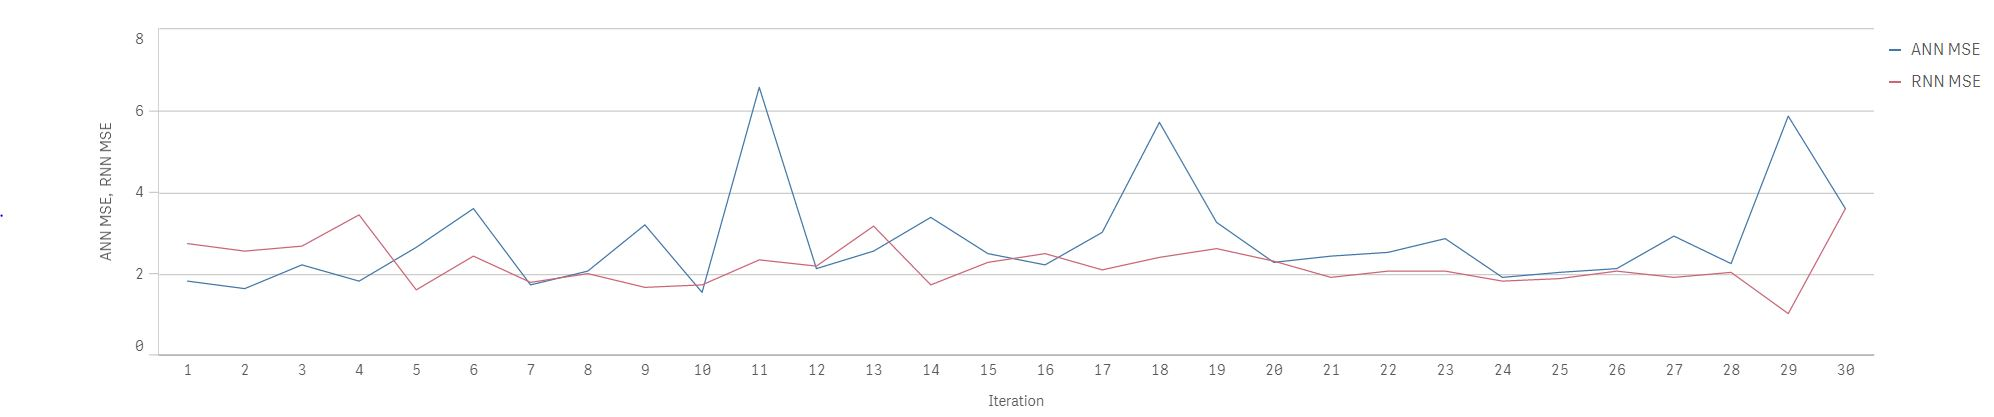
\includegraphics[width=13cm,height=7cm]{Figures/errors.JPG}
\caption{ANN MSE vs. RNN MSE}
\end{figure}

 
 

 
 
